\documentclass[]{article}
\usepackage{lmodern}
\usepackage{amssymb,amsmath}
\usepackage{ifxetex,ifluatex}
\usepackage{fixltx2e} % provides \textsubscript
\ifnum 0\ifxetex 1\fi\ifluatex 1\fi=0 % if pdftex
  \usepackage[T1]{fontenc}
  \usepackage[utf8]{inputenc}
\else % if luatex or xelatex
  \ifxetex
    \usepackage{mathspec}
  \else
    \usepackage{fontspec}
  \fi
  \defaultfontfeatures{Ligatures=TeX,Scale=MatchLowercase}
\fi
% use upquote if available, for straight quotes in verbatim environments
\IfFileExists{upquote.sty}{\usepackage{upquote}}{}
% use microtype if available
\IfFileExists{microtype.sty}{%
\usepackage{microtype}
\UseMicrotypeSet[protrusion]{basicmath} % disable protrusion for tt fonts
}{}
\usepackage[margin=1in]{geometry}
\usepackage{hyperref}
\hypersetup{unicode=true,
            pdftitle={Lab 11},
            pdfborder={0 0 0},
            breaklinks=true}
\urlstyle{same}  % don't use monospace font for urls
\usepackage{color}
\usepackage{fancyvrb}
\newcommand{\VerbBar}{|}
\newcommand{\VERB}{\Verb[commandchars=\\\{\}]}
\DefineVerbatimEnvironment{Highlighting}{Verbatim}{commandchars=\\\{\}}
% Add ',fontsize=\small' for more characters per line
\usepackage{framed}
\definecolor{shadecolor}{RGB}{248,248,248}
\newenvironment{Shaded}{\begin{snugshade}}{\end{snugshade}}
\newcommand{\KeywordTok}[1]{\textcolor[rgb]{0.13,0.29,0.53}{\textbf{{#1}}}}
\newcommand{\DataTypeTok}[1]{\textcolor[rgb]{0.13,0.29,0.53}{{#1}}}
\newcommand{\DecValTok}[1]{\textcolor[rgb]{0.00,0.00,0.81}{{#1}}}
\newcommand{\BaseNTok}[1]{\textcolor[rgb]{0.00,0.00,0.81}{{#1}}}
\newcommand{\FloatTok}[1]{\textcolor[rgb]{0.00,0.00,0.81}{{#1}}}
\newcommand{\ConstantTok}[1]{\textcolor[rgb]{0.00,0.00,0.00}{{#1}}}
\newcommand{\CharTok}[1]{\textcolor[rgb]{0.31,0.60,0.02}{{#1}}}
\newcommand{\SpecialCharTok}[1]{\textcolor[rgb]{0.00,0.00,0.00}{{#1}}}
\newcommand{\StringTok}[1]{\textcolor[rgb]{0.31,0.60,0.02}{{#1}}}
\newcommand{\VerbatimStringTok}[1]{\textcolor[rgb]{0.31,0.60,0.02}{{#1}}}
\newcommand{\SpecialStringTok}[1]{\textcolor[rgb]{0.31,0.60,0.02}{{#1}}}
\newcommand{\ImportTok}[1]{{#1}}
\newcommand{\CommentTok}[1]{\textcolor[rgb]{0.56,0.35,0.01}{\textit{{#1}}}}
\newcommand{\DocumentationTok}[1]{\textcolor[rgb]{0.56,0.35,0.01}{\textbf{\textit{{#1}}}}}
\newcommand{\AnnotationTok}[1]{\textcolor[rgb]{0.56,0.35,0.01}{\textbf{\textit{{#1}}}}}
\newcommand{\CommentVarTok}[1]{\textcolor[rgb]{0.56,0.35,0.01}{\textbf{\textit{{#1}}}}}
\newcommand{\OtherTok}[1]{\textcolor[rgb]{0.56,0.35,0.01}{{#1}}}
\newcommand{\FunctionTok}[1]{\textcolor[rgb]{0.00,0.00,0.00}{{#1}}}
\newcommand{\VariableTok}[1]{\textcolor[rgb]{0.00,0.00,0.00}{{#1}}}
\newcommand{\ControlFlowTok}[1]{\textcolor[rgb]{0.13,0.29,0.53}{\textbf{{#1}}}}
\newcommand{\OperatorTok}[1]{\textcolor[rgb]{0.81,0.36,0.00}{\textbf{{#1}}}}
\newcommand{\BuiltInTok}[1]{{#1}}
\newcommand{\ExtensionTok}[1]{{#1}}
\newcommand{\PreprocessorTok}[1]{\textcolor[rgb]{0.56,0.35,0.01}{\textit{{#1}}}}
\newcommand{\AttributeTok}[1]{\textcolor[rgb]{0.77,0.63,0.00}{{#1}}}
\newcommand{\RegionMarkerTok}[1]{{#1}}
\newcommand{\InformationTok}[1]{\textcolor[rgb]{0.56,0.35,0.01}{\textbf{\textit{{#1}}}}}
\newcommand{\WarningTok}[1]{\textcolor[rgb]{0.56,0.35,0.01}{\textbf{\textit{{#1}}}}}
\newcommand{\AlertTok}[1]{\textcolor[rgb]{0.94,0.16,0.16}{{#1}}}
\newcommand{\ErrorTok}[1]{\textcolor[rgb]{0.64,0.00,0.00}{\textbf{{#1}}}}
\newcommand{\NormalTok}[1]{{#1}}
\usepackage{graphicx,grffile}
\makeatletter
\def\maxwidth{\ifdim\Gin@nat@width>\linewidth\linewidth\else\Gin@nat@width\fi}
\def\maxheight{\ifdim\Gin@nat@height>\textheight\textheight\else\Gin@nat@height\fi}
\makeatother
% Scale images if necessary, so that they will not overflow the page
% margins by default, and it is still possible to overwrite the defaults
% using explicit options in \includegraphics[width, height, ...]{}
\setkeys{Gin}{width=\maxwidth,height=\maxheight,keepaspectratio}
\IfFileExists{parskip.sty}{%
\usepackage{parskip}
}{% else
\setlength{\parindent}{0pt}
\setlength{\parskip}{6pt plus 2pt minus 1pt}
}
\setlength{\emergencystretch}{3em}  % prevent overfull lines
\providecommand{\tightlist}{%
  \setlength{\itemsep}{0pt}\setlength{\parskip}{0pt}}
\setcounter{secnumdepth}{0}
% Redefines (sub)paragraphs to behave more like sections
\ifx\paragraph\undefined\else
\let\oldparagraph\paragraph
\renewcommand{\paragraph}[1]{\oldparagraph{#1}\mbox{}}
\fi
\ifx\subparagraph\undefined\else
\let\oldsubparagraph\subparagraph
\renewcommand{\subparagraph}[1]{\oldsubparagraph{#1}\mbox{}}
\fi

%%% Use protect on footnotes to avoid problems with footnotes in titles
\let\rmarkdownfootnote\footnote%
\def\footnote{\protect\rmarkdownfootnote}

%%% Change title format to be more compact
\usepackage{titling}

% Create subtitle command for use in maketitle
\newcommand{\subtitle}[1]{
  \posttitle{
    \begin{center}\large#1\end{center}
    }
}

\setlength{\droptitle}{-2em}
  \title{Lab 11}
  \pretitle{\vspace{\droptitle}\centering\huge}
  \posttitle{\par}
  \author{}
  \preauthor{}\postauthor{}
  \predate{\centering\large\emph}
  \postdate{\par}
  \date{November 17, 2016}


\begin{document}
\maketitle

This is an \href{http://rmarkdown.rstudio.com}{R Markdown} Notebook.

\subsection{More on numerical stability of Importance
Sampling}\label{more-on-numerical-stability-of-importance-sampling}

When calculating the likelihood for a large sample you, the likelihood
will often take on astronomically small values, so numerical
considerations must be taken. For example, R would conclude the quantity

\[\frac{e^{-1000}}{e^{-1000}+e^{-1001}}\]

is \texttt{NaN}, because both the numerator and denominator are both 0,
as far as R is concerned.

\begin{Shaded}
\begin{Highlighting}[]
\KeywordTok{exp}\NormalTok{(-}\DecValTok{1000}\NormalTok{)/(}\KeywordTok{exp}\NormalTok{(-}\DecValTok{1000}\NormalTok{)+}\KeywordTok{exp}\NormalTok{(-}\DecValTok{1001}\NormalTok{))}
\end{Highlighting}
\end{Shaded}

\begin{verbatim}
## [1] NaN
\end{verbatim}

However, we know this quantity is equal to \(1/(1 + e^{-1}) = .731\).

\begin{Shaded}
\begin{Highlighting}[]
\DecValTok{1}\NormalTok{/(}\DecValTok{1}\NormalTok{+}\KeywordTok{exp}\NormalTok{(-}\DecValTok{1}\NormalTok{))}
\end{Highlighting}
\end{Shaded}

\begin{verbatim}
## [1] 0.7310586
\end{verbatim}

The importance function has a similar issue, since it is a ratio of two
densities. It is numerically more stable to work with
\[\mathrm{log}(\tilde{w}(x)) = \mathrm{log}(\tilde\pi(x))-\mathrm{log}(g(x))\]
This is necessary when the sample size is relatively large. Let
\[M = \max_i \mathrm{log}(\tilde{w}(Xi))\] we can derive the new
estimator:

\[
\begin{aligned}
\overline{\pi_{n, IS}}(h) 
&= \frac{\sum_{k=1}^n{h(X_k)\tilde{\omega}(X_k)}}{\sum_{k=1}^n{\tilde{\omega}(X_k)}}\\
&= \frac{\sum_{k=1}^n{h(X_k)\exp(\log(\tilde{\omega}(X_k)))}}{\sum_{k=1}^n{\exp(\log(\tilde{\omega}(X_k)))}}\\
&= \frac{e^M\sum_{k=1}^n{h(X_k)\exp(\log(\tilde{\omega}(X_k))-M)}}{e^M\sum_{k=1}^n{\exp(\log(\tilde{\omega}(X_k))-M)}}\\
&= \frac{\sum_{k=1}^n{h(X_k)\exp(\log(\tilde{\omega}(X_k))-M)}}{\sum_{k=1}^n{\exp(\log(\tilde{\omega}(X_k))-M)}}\\
\end{aligned}
\] The final line is a more numerically stable version of the importance
sampling estimator.

The famed Bayes Theorem:

\subsection{Bayes theorem and old
western}\label{bayes-theorem-and-old-western}

The following is an abridged version of the same story detailed on
\href{https://books.google.com/books?id=JWLIRr_ROgAC\&pg=PA155\#v=onepage\&q\&f=false}{page
155 of \textbf{The Cult of Statistical Significance}}:

Dolores arrives at Sweetwater town trying to find out how Arnold died.
Without a body to inspect, classical inference is of little help to her:

Classical hypothesis testing evaluates the hypothesis ``Arnold was
hanged'' based on the likelihood of the outcome of the hypothesis.
Usually it is impossible to escape death if you are hanged (unless you
are in an old western), so the hypothesis is not implausible.

Then Dolores remembers he could also have caught pneumonia, or a bullet;
each of those hypotheses cannot be rejected either. With a millions ways
to die in the west, she is left scatching her head.

Fisher's test evaluates the probability of Arnold is dead, given that he
was hanged (\(P(\mbox{D}|\mbox{H})\)). What she wants to know is the
opposite: the probability of he hanged, given that he is now dead
(\(P(\mbox{H}|\mbox{D})\)).

\subsubsection{Bayes to the rescue}\label{bayes-to-the-rescue}

If she understands Bayes theorem, and some context of the world they
live in, things can become easier.

In a world where people die from dehydration, cattle stampedes, bullet
wounds, flu, and cardiac arrest, being dead is very weak evidence that
the person was hanged. When the probability of being hanged is low
compared to other ailments to start with, the probability of him dying
from hanging, after knowing the outcome, can still be small.

\paragraph{But wait, there's more}\label{but-wait-theres-more}

It is not coincidental that the author of the book chose to name the
hypothesis ``hanging'', and data ``death''. But we don't have to. We can
in fact calculate the probability of each hypothesis.

\[ P(\mbox{H}=i|\mbox{D}) = \frac{P(\mbox{D}|\mbox{H}=i)P(\mbox{H}=i)}{P(\mbox{D})} \]

Hence we know the ratio of the probability of any two hypothesis, ex
post facto, quite easily:

\[
\frac{P(\mbox{H}=i|\mbox{D})}{P(\mbox{H}=j|\mbox{D})} 
= \frac{P(\mbox{D}|\mbox{H}=i)P(\mbox{H}=i)}{P(\mbox{D})} \frac{P(\mbox{D})}{P(\mbox{D}|\mbox{H}=j)P(\mbox{H}=j)} 
= \frac{P(\mbox{D}|\mbox{H}=i)P(\mbox{H}=i)}{P(\mbox{D}|\mbox{H}=j)P(\mbox{H}=j)}
\]

That is,

\[
P(\mbox{H}=i|\mbox{D}) \propto P(\mbox{D}|\mbox{H}=i)P(\mbox{H}=i)
\]

and \(P(\mbox{D})\) is a normalizing constant that does not vary with
your hypothesis.

Knowing the probability sums to 1,

\[P(\mbox{D}) = \sum_i P(\mbox{D}|\mbox{H}=i)P(\mbox{H}=i)\]

\subsubsection{Naming conventions}\label{naming-conventions}

We call the \(P(\mbox{H})\) the prior (prior belief, before observing
the data), \(P(\mbox{H}|\mbox{D})\) the posterior, and
\(P(\mbox{D}|\mbox{H})\) the likelihood.

Posterior is proportional to the likelihood times the prior.

Common notations:

\begin{itemize}
\tightlist
\item
  \(\Theta\) for parameter of interest
\item
  \(Y\) for random event observed
\item
  \(\pi(\theta)\) the prior
\item
  \(f(y|\theta)\) the likelihood
\item
  \(\pi(\theta|y)\) the posterior
\end{itemize}

\section{Bayesian Inference}\label{bayesian-inference}

The primary examples where you want to determine properties of a
distribution given only the unnormalized density come from Bayesian
inference. Suppose you observe data \(y_1, ..., y_n\) with density
\(f(y|\theta)\) indexed by a parameter \(\theta\). A typical approach is
to view \(\theta\) as a fixed unknown truth you want to determine and
and estimate by maximum likelihood

\[\max_\theta f_\theta(y_1, ..., y_n)\] Instead, a bayesian approach
views the parameter as having a distribution when conditioned on the
data, and look to make inference about the posterior density,
\(\pi(\theta|y_1, ..., y_n)\). Noting that \(f_\theta(y) = f(y|\theta)\)
and applying bayes rule twice: \[
\pi(\theta|y_1, ..., y_n) = \frac{p(\theta, y_1, ..., y_n)}{p(y_1, ..., y_n)} = \frac{f(y_1, ..., y_n|\theta)\pi(\theta)}{p(y_1, ..., y_n)}
\] In the case of \(y_i\)'s being iid samples, as the sample size
increases, the shape of the posterior is increasingly dominated by the
likelihood.

The denominator, i.e., the marginal probability of the data
\[p(y_1, ..., y_n) = \int p(\theta, y_1, ..., y_n)\mathrm{d}\theta = \int f(y_1, ..., y_n|\theta)\pi(\theta)\mathrm{d}\theta\]

is the normalizing constant for the posterior distribution and is often
an intractable integral. We can apply importance sampling to the
unnormalized posterior density \[f(y_1, ..., y_n|\theta)\pi(\theta)\]

\subsubsection{Example 1}\label{example-1}

Suppose \(X_1, ..., X_n \sim \mathrm{Binomial}(10, \theta)\) where
\(\theta \in (0, 1)\) has a \(\mathrm{Beta}(5, 3)\) prior density: \[
\pi(\theta) = \frac{\Gamma(8)}{\Gamma(5)\Gamma(3)}\theta^4(1-\theta)^2
\] We want to estimate the mean of the posterior distribution:
\(\int\theta\pi(\theta|x_1, ..., x_n)\mathrm{d}\theta\). Take the
(proposal) density function g in importance sampling to be
\(\mathrm{Beta}(\alpha, \beta)\) density, where \[
\alpha = c\bar{X}\\
\beta = c(10 - \bar{X})
\] where \(\bar{X}\) is the sample mean, and c is a positive constant.
This will ensure that g is peaked near the MLE \(\bar{X}/10\), where the
posterior distribution should have a lot of mass. The larger c is, the
more sharply peaked around \(\bar{X}/10\) will be. We will tune c to
minimize the variance of the estimate.

Likelihood:

\[
\begin{aligned}
f(x_1, ... , x_n|\theta) 
&= \prod_{i=1}^nf(x_i|\theta)\\
&= \prod_{i=1}^n\binom{10}{x_i}\theta^{x_i}(1-\theta)^{10-x_i}\\
&\propto \theta^{\sum x_i}(1-\theta)^{10-\sum x_i}\\
&= \theta^{n\bar{x}}(1-\theta)^{n(10-\bar{x})}\\
\end{aligned}
\]

Posterior:

\[
\begin{aligned}
\pi(\theta|x_1, ... , x_n)
&\propto f(x_1, ... , x_n|\theta) \pi(\theta)\\
&\propto \theta^{n\bar{x}}(1-\theta)^{n(10-\bar{x})} \pi(\theta)\\
&= \theta^{n\bar{x}}(1-\theta)^{n(10-\bar{x})} \frac{\Gamma(8)}{\Gamma(5)\Gamma(3)}\theta^4(1-\theta)^2\\
&\propto \theta^{n\bar{x}}(1-\theta)^{n(10-\bar{x})} \theta^4(1-\theta)^2\\
&= \theta^{n\bar{x}+4}(1-\theta)^{n(10-\bar{x})+2}
\end{aligned}
\]

The log of this quantity is \[
{(n\bar{x}+4)}\log(\theta) + {(n(10-\bar{x})+2)}\log(1-\theta)
\]

The following code illuistrate choices of different trial/proposal
densities to approximate posterior.

\begin{Shaded}
\begin{Highlighting}[]
\NormalTok{log.prior <-}\StringTok{  }\NormalTok{function(theta) \{}
  \DecValTok{4} \NormalTok{*}\StringTok{ }\KeywordTok{log}\NormalTok{(theta) +}\StringTok{ }\DecValTok{2} \NormalTok{*}\StringTok{ }\KeywordTok{log}\NormalTok{(}\DecValTok{1} \NormalTok{-}\StringTok{ }\NormalTok{theta)}
\NormalTok{\}}

\NormalTok{log.likelihood <-}\StringTok{  }\NormalTok{function(data, theta) \{}
  \NormalTok{n <-}\StringTok{ }\KeywordTok{length}\NormalTok{(data)}
  \KeywordTok{sum}\NormalTok{(data) *}\StringTok{ }\KeywordTok{log}\NormalTok{(theta) +}\StringTok{ }\NormalTok{n *}\StringTok{ }\NormalTok{(}\DecValTok{10} \NormalTok{-}\StringTok{ }\KeywordTok{mean}\NormalTok{(data)) *}\StringTok{ }\KeywordTok{log}\NormalTok{(}\DecValTok{1} \NormalTok{-}\StringTok{ }\NormalTok{theta)}
\NormalTok{\}}

\NormalTok{log.posterior <-}\StringTok{  }\NormalTok{function(data, theta) \{}
  \KeywordTok{log.prior}\NormalTok{(theta) +}\StringTok{ }\KeywordTok{log.likelihood}\NormalTok{(data, theta)}
\NormalTok{\}}

\NormalTok{log.g <-}\StringTok{ }\NormalTok{function(data, theta, C) \{}
   \KeywordTok{dbeta}\NormalTok{(theta, C *}\StringTok{ }\KeywordTok{mean}\NormalTok{(data), C *}\StringTok{ }\NormalTok{(}\DecValTok{10} \NormalTok{-}\StringTok{ }\KeywordTok{mean}\NormalTok{(data)), }\DataTypeTok{log =} \OtherTok{TRUE}\NormalTok{)}
\NormalTok{\}}

\NormalTok{data =}\StringTok{ }\KeywordTok{rbinom}\NormalTok{(}\DecValTok{10}\NormalTok{, }\DecValTok{10}\NormalTok{, .}\DecValTok{4}\NormalTok{)}

\NormalTok{theta.seq <-}\StringTok{ }\KeywordTok{seq}\NormalTok{(}\DecValTok{0}\NormalTok{,}\DecValTok{1}\NormalTok{,}\FloatTok{0.001}\NormalTok{)}
\NormalTok{log.prior.eval <-}\StringTok{ }\KeywordTok{log.prior}\NormalTok{(theta.seq)}
\NormalTok{log.likelihood.eval <-}\StringTok{ }\KeywordTok{log.likelihood}\NormalTok{(data, theta.seq)}
\NormalTok{log.posterior.eval <-}\StringTok{ }\KeywordTok{log.posterior}\NormalTok{(data, theta.seq)}

\KeywordTok{plot}\NormalTok{(theta.seq, }\KeywordTok{exp}\NormalTok{(log.prior.eval-}\KeywordTok{max}\NormalTok{(log.prior.eval)),}
     \DataTypeTok{type =} \StringTok{'l'}\NormalTok{, }\DataTypeTok{xlab =} \StringTok{"theta"}\NormalTok{, }\DataTypeTok{ylab =} \StringTok{"density up to normalization"}\NormalTok{,}
     \DataTypeTok{main =} \StringTok{"Prior and posterior densities"}\NormalTok{)}
\KeywordTok{lines}\NormalTok{(theta.seq, }\KeywordTok{exp}\NormalTok{(log.likelihood.eval-}\KeywordTok{max}\NormalTok{(log.likelihood.eval)), }\DataTypeTok{col =} \DecValTok{2}\NormalTok{)}
\KeywordTok{lines}\NormalTok{(theta.seq, }\KeywordTok{exp}\NormalTok{(log.posterior.eval-}\KeywordTok{max}\NormalTok{(log.posterior.eval)), }\DataTypeTok{col =} \DecValTok{3}\NormalTok{)}
\KeywordTok{legend}\NormalTok{(}\StringTok{"topleft"}\NormalTok{, }\DataTypeTok{legend =} \KeywordTok{c}\NormalTok{(}\StringTok{"Prior"}\NormalTok{, }\StringTok{"Likelihood"}\NormalTok{, }\StringTok{"Posterior"}\NormalTok{),}
       \DataTypeTok{lty =} \DecValTok{1}\NormalTok{, }\DataTypeTok{col =} \KeywordTok{c}\NormalTok{(}\DecValTok{1}\NormalTok{:}\DecValTok{3}\NormalTok{))}
\end{Highlighting}
\end{Shaded}

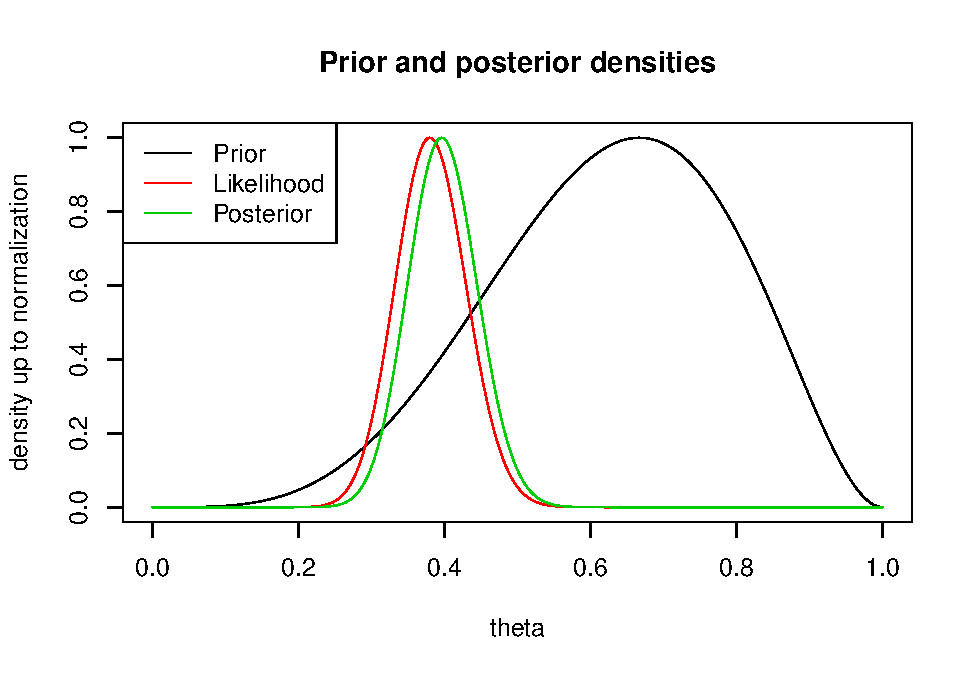
\includegraphics{Stats406Lab11_files/figure-latex/unnamed-chunk-3-1.pdf}

\begin{Shaded}
\begin{Highlighting}[]
\NormalTok{C.choice1 <-}\StringTok{ }\DecValTok{1}
\NormalTok{C.choice2 <-}\StringTok{ }\DecValTok{10}
\NormalTok{C.choice3 <-}\StringTok{ }\DecValTok{50}
\NormalTok{log.g1.eval <-}\StringTok{ }\KeywordTok{log.g}\NormalTok{(data, theta.seq, C.choice1)}
\NormalTok{log.g2.eval <-}\StringTok{ }\KeywordTok{log.g}\NormalTok{(data, theta.seq, C.choice2)}
\NormalTok{log.g3.eval <-}\StringTok{ }\KeywordTok{log.g}\NormalTok{(data, theta.seq, C.choice3)}

\KeywordTok{plot}\NormalTok{(theta.seq, }\KeywordTok{exp}\NormalTok{(log.posterior.eval-}\KeywordTok{max}\NormalTok{(log.posterior.eval)),}
     \DataTypeTok{type =} \StringTok{'l'}\NormalTok{, }\DataTypeTok{xlab =} \StringTok{"theta"}\NormalTok{, }\DataTypeTok{ylab =} \StringTok{"density up to normalization"}\NormalTok{,}
     \DataTypeTok{main =} \StringTok{"Posterior and proposal densities"}\NormalTok{, }\DataTypeTok{col =} \DecValTok{3}\NormalTok{, }\DataTypeTok{lwd =} \DecValTok{2}\NormalTok{)}
\KeywordTok{lines}\NormalTok{(theta.seq, }\KeywordTok{exp}\NormalTok{(log.g1.eval-}\KeywordTok{max}\NormalTok{(log.g1.eval)), }\DataTypeTok{col =} \DecValTok{4}\NormalTok{, }\DataTypeTok{lty =} \DecValTok{2}\NormalTok{)}
\KeywordTok{lines}\NormalTok{(theta.seq, }\KeywordTok{exp}\NormalTok{(log.g2.eval-}\KeywordTok{max}\NormalTok{(log.g2.eval)), }\DataTypeTok{col =} \DecValTok{4}\NormalTok{, }\DataTypeTok{lty =} \DecValTok{3}\NormalTok{)}
\KeywordTok{lines}\NormalTok{(theta.seq, }\KeywordTok{exp}\NormalTok{(log.g3.eval-}\KeywordTok{max}\NormalTok{(log.g3.eval)), }\DataTypeTok{col =} \DecValTok{4}\NormalTok{, }\DataTypeTok{lty =} \DecValTok{4}\NormalTok{)}

\KeywordTok{legend}\NormalTok{(}\StringTok{"topright"}\NormalTok{, }\DataTypeTok{legend =} \KeywordTok{c}\NormalTok{(}\StringTok{"Posterior"}\NormalTok{, }\StringTok{"Proposal 1"}\NormalTok{, }\StringTok{"Proposal 2"}\NormalTok{, }\StringTok{"Proposal 3"}\NormalTok{),}
       \DataTypeTok{lty =} \DecValTok{1}\NormalTok{:}\DecValTok{4}\NormalTok{, }\DataTypeTok{col =} \KeywordTok{c}\NormalTok{(}\DecValTok{3}\NormalTok{,}\DecValTok{4}\NormalTok{,}\DecValTok{4}\NormalTok{,}\DecValTok{4}\NormalTok{))}
\end{Highlighting}
\end{Shaded}

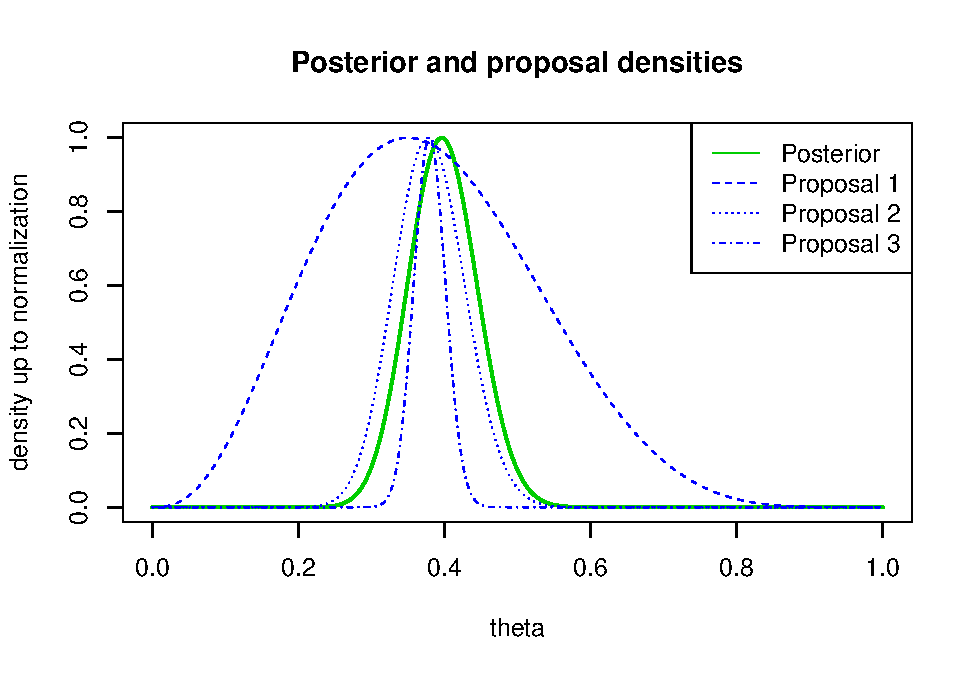
\includegraphics{Stats406Lab11_files/figure-latex/unnamed-chunk-3-2.pdf}

The bettter our proposal density approximates the posterior density, the
less variable the importance weight \(\pi(\theta|data)/g(\theta)\),
hence the more accurate our importance sampling estimates will be.

The following R code executes the importance sampling:

\begin{Shaded}
\begin{Highlighting}[]
\CommentTok{# X is the data, res is the number of monte carlo samples,}
\CommentTok{# C is the tuning parameter for the g distribution}
\NormalTok{IS <-}\StringTok{ }\NormalTok{function(X, C, n)}
\NormalTok{\{}
  \CommentTok{# sample size}
  \NormalTok{n <-}\StringTok{ }\KeywordTok{length}\NormalTok{(X)}
  \CommentTok{# log posterior derived above}
  \NormalTok{log.posterior <-}\StringTok{  }\NormalTok{function(theta) \{}
    \NormalTok{(}\KeywordTok{sum}\NormalTok{(X) +}\StringTok{ }\DecValTok{4}\NormalTok{) *}\StringTok{ }\KeywordTok{log}\NormalTok{(theta) +}\StringTok{ }\NormalTok{(n *}\StringTok{ }\NormalTok{(}\DecValTok{10} \NormalTok{-}\StringTok{ }\KeywordTok{mean}\NormalTok{(X)) +}\StringTok{ }\DecValTok{2}\NormalTok{) *}\StringTok{ }\KeywordTok{log}\NormalTok{(}\DecValTok{1} \NormalTok{-}\StringTok{ }\NormalTok{theta)}
  \NormalTok{\}}
  \CommentTok{# log trial (proposal) density, g}
  \NormalTok{log.g <-}\StringTok{ }\NormalTok{function(theta) \{}
    \KeywordTok{dbeta}\NormalTok{(theta, C *}\StringTok{ }\KeywordTok{mean}\NormalTok{(X), C *}\StringTok{ }\NormalTok{(}\DecValTok{10} \NormalTok{-}\StringTok{ }\KeywordTok{mean}\NormalTok{(X)), }\DataTypeTok{log =} \OtherTok{TRUE}\NormalTok{)}
  \NormalTok{\}}
  
  \CommentTok{# log importance function}
  \NormalTok{log.w <-}\StringTok{ }\NormalTok{function(theta) \{}
    \KeywordTok{log.posterior}\NormalTok{(theta) -}\StringTok{ }\KeywordTok{log.g}\NormalTok{(theta)}
  \NormalTok{\}}
  
  \CommentTok{# generate from the trial (proposal) distribution}
  \NormalTok{U <-}\StringTok{ }\KeywordTok{rbeta}\NormalTok{(n, C *}\StringTok{ }\KeywordTok{mean}\NormalTok{(X), C *}\StringTok{ }\NormalTok{(}\DecValTok{10} \NormalTok{-}\StringTok{ }\KeywordTok{mean}\NormalTok{(X)))}
  
  \CommentTok{# calculate the list of log.w values}
  \NormalTok{LP <-}\StringTok{ }\KeywordTok{log.w}\NormalTok{(U)}
  
  \CommentTok{# factor out the largest value to prevent numerical underflow}
  \NormalTok{w <-}\StringTok{ }\KeywordTok{max}\NormalTok{(LP)}
  \NormalTok{LP <-}\StringTok{ }\NormalTok{LP -}\StringTok{ }\NormalTok{w}
  
  \CommentTok{# importance sampling estimate}
  \NormalTok{I <-}\StringTok{ }\KeywordTok{mean}\NormalTok{(}\KeywordTok{exp}\NormalTok{(LP) *}\StringTok{ }\NormalTok{U) /}\StringTok{ }\KeywordTok{mean}\NormalTok{(}\KeywordTok{exp}\NormalTok{(LP))}
  
  \CommentTok{# calculate CV}
  \NormalTok{CV <-}\StringTok{ }\KeywordTok{sqrt}\NormalTok{( }\KeywordTok{var}\NormalTok{( }\KeywordTok{exp}\NormalTok{(LP) /}\StringTok{ }\KeywordTok{mean}\NormalTok{(}\KeywordTok{exp}\NormalTok{(LP) ) ) )}
  
  \CommentTok{# calculate s.e. of the IS estimate}
  \NormalTok{Z =}\StringTok{ }\KeywordTok{exp}\NormalTok{(LP) *}\StringTok{ }\NormalTok{U /}\StringTok{ }\KeywordTok{mean}\NormalTok{(}\KeywordTok{exp}\NormalTok{(LP))}
  \NormalTok{sig.sq <-}\StringTok{ }\KeywordTok{var}\NormalTok{( Z )}
  \NormalTok{se <-}\StringTok{ }\KeywordTok{sqrt}\NormalTok{( sig.sq /}\StringTok{ }\NormalTok{n )}
  
  \CommentTok{# return the 95 percent confidence interval for the estimate}
  \KeywordTok{return}\NormalTok{(}\KeywordTok{list}\NormalTok{(}\DataTypeTok{lower =} \NormalTok{I -}\StringTok{ }\FloatTok{1.96} \NormalTok{*}\StringTok{ }\NormalTok{se, }\DataTypeTok{upper =} \NormalTok{I +}\StringTok{ }\FloatTok{1.96} \NormalTok{*}\StringTok{ }\NormalTok{se, }\DataTypeTok{CV =} \NormalTok{CV))}
\NormalTok{\}}

\CommentTok{# Generate 100 binomial(10,.4) random variables}
\NormalTok{X =}\StringTok{ }\KeywordTok{rbinom}\NormalTok{(}\DecValTok{100}\NormalTok{, }\DecValTok{10}\NormalTok{, .}\DecValTok{4}\NormalTok{)}

\NormalTok{## calculate CV and var(E(theta|X))}
\NormalTok{## over a grid of values for alpha}
\NormalTok{C <-}\StringTok{ }\KeywordTok{seq}\NormalTok{(.}\DecValTok{1}\NormalTok{, }\DecValTok{200}\NormalTok{, }\DataTypeTok{length =} \DecValTok{2000}\NormalTok{)}
\NormalTok{A <-}\StringTok{ }\KeywordTok{matrix}\NormalTok{(}\DecValTok{0}\NormalTok{, }\DecValTok{2000}\NormalTok{, }\DecValTok{2}\NormalTok{)}

\NormalTok{for (j in }\DecValTok{1}\NormalTok{:}\DecValTok{2000}\NormalTok{) \{}
  \NormalTok{output <-}\StringTok{ }\KeywordTok{IS}\NormalTok{(X, C[j], }\DecValTok{1000}\NormalTok{)}
  \NormalTok{CV <-}\StringTok{ }\NormalTok{output$CV}
  \NormalTok{V <-}\StringTok{ }\NormalTok{(output$upper -}\StringTok{ }\NormalTok{output$lower) /}\StringTok{ }\FloatTok{3.92}
  \NormalTok{A[j, ] <-}\StringTok{ }\KeywordTok{c}\NormalTok{(CV, V)}
\NormalTok{\}}

\CommentTok{# see where CV is low enough}
\KeywordTok{plot}\NormalTok{(C, A[, }\DecValTok{1}\NormalTok{], }\DataTypeTok{ylab =} \StringTok{"CV"}\NormalTok{, }\DataTypeTok{xlab =} \StringTok{"c"}\NormalTok{,}
     \DataTypeTok{main =} \StringTok{"CV vs. c"}\NormalTok{, }\DataTypeTok{col =} \DecValTok{2}\NormalTok{, }\DataTypeTok{type =} \StringTok{"l"}\NormalTok{)}
\KeywordTok{abline}\NormalTok{(}\DataTypeTok{h =} \DecValTok{5}\NormalTok{)}
\end{Highlighting}
\end{Shaded}

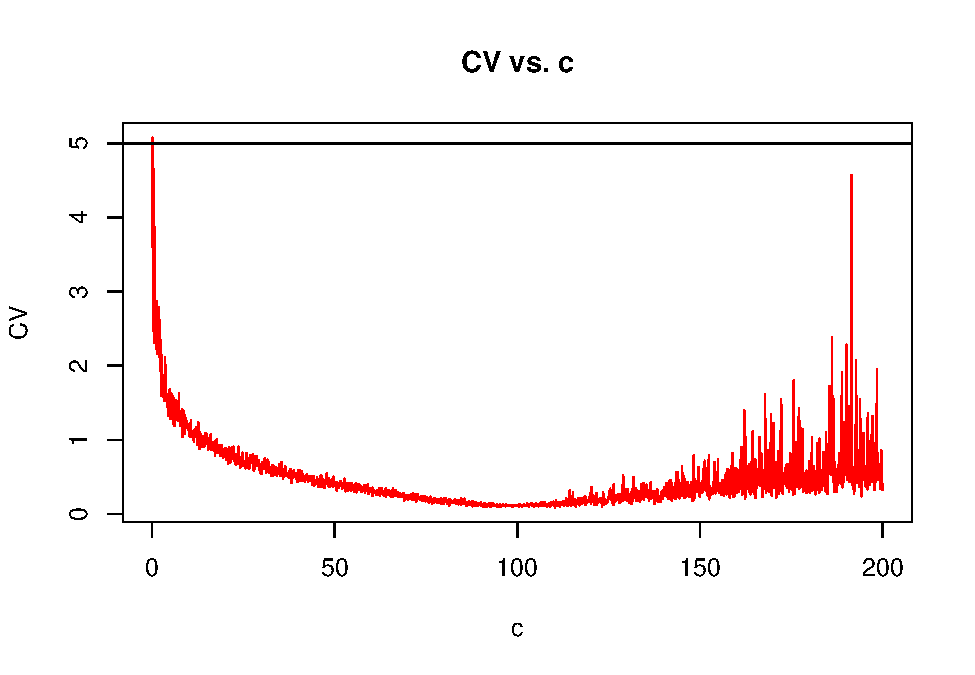
\includegraphics{Stats406Lab11_files/figure-latex/unnamed-chunk-4-1.pdf}

\begin{Shaded}
\begin{Highlighting}[]
\CommentTok{# standard error estimates}
\KeywordTok{plot}\NormalTok{(C, A[, }\DecValTok{2}\NormalTok{], }\DataTypeTok{xlab =} \StringTok{"c"}\NormalTok{, }\DataTypeTok{ylab =} \StringTok{"Standard error estimate"}\NormalTok{,}
     \DataTypeTok{main =} \StringTok{"se vs. c"}\NormalTok{, }\DataTypeTok{col =} \DecValTok{4}\NormalTok{, }\DataTypeTok{type =} \StringTok{"l"}\NormalTok{)}
\end{Highlighting}
\end{Shaded}

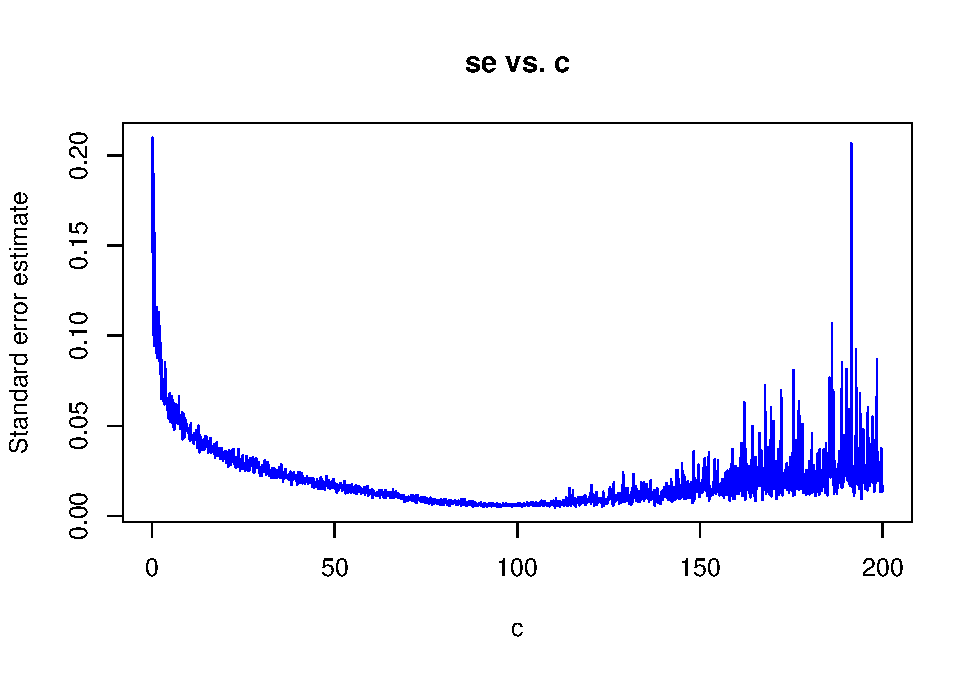
\includegraphics{Stats406Lab11_files/figure-latex/unnamed-chunk-4-2.pdf}

\begin{Shaded}
\begin{Highlighting}[]
\CommentTok{# The final confidence interval}
\KeywordTok{IS}\NormalTok{(X, C[}\KeywordTok{which.min}\NormalTok{(A[, }\DecValTok{2}\NormalTok{])], }\DecValTok{1000}\NormalTok{)[}\DecValTok{1}\NormalTok{:}\DecValTok{2}\NormalTok{]}
\end{Highlighting}
\end{Shaded}

\begin{verbatim}
## $lower
## [1] 0.388266
## 
## $upper
## [1] 0.4237535
\end{verbatim}

\subsection{Bootstrap}\label{bootstrap}

Suppose we want to estimate a parameter \(\theta\) of the population
distribution \(\mathcal{F}\). We propose an estimator \(\hat\theta\)
based on a collected samples \(\mathcal{X} = {X_1 , ... , X_n}\).

We want know how good \(\hat\theta\) is by evaluating
\(\mathrm{MSE}(\hat\theta)\).

If we know \(\mathcal{F}\), then in principle we can calculate
\(\mathrm{MSE}(\hat\theta)\). But unless the distribution is easy to
handle (e.g.~normal), analytical formulation is intractable. Besides, we
do not know \(\mathcal{F}\) in practice.

Suppose we can sample from F, how to compute
\(\mathrm{MSE}(\hat\theta)\)?

\begin{enumerate}
\def\labelenumi{\arabic{enumi}.}
\tightlist
\item
  Draw samples \(\mathcal{X}_1 , ... , \mathcal{X}_K\), each of size
  \(n\), from \(\mathcal{F}_\theta\).
\item
  Compute sample statistic \(\hat\theta_k\) for each sample
  \(\mathcal{X}_k\).
\item
  Approximate MSE of \(\theta\) by
  \(\sum_{k=1}^K (\hat\theta_k - \theta)^2/n\) .
\end{enumerate}

Bootstrap: Now we don’t know F, and have only one sample
\(\mathcal{X}\), we can mimic the above procedure

\begin{enumerate}
\def\labelenumi{\arabic{enumi}.}
\tightlist
\item
  Draw bootstrap samples \(\mathcal{X}_1^* , ... , \mathcal{X}_K^*\),
  each of size \(n\), from the original sample \(\mathcal{X}\).
\item
  Compute sample statistic \(\hat\theta_k^*\) for each sample
  \(\mathcal{X}_k^*\).
\item
  Aprroximate MSE of \(\theta\) by
  \(\sum_{k=1}^K (\hat\theta_k^* - \hat\theta)^2/n\), where
  \(\hat\theta\) is the estimate from original sample \(\mathcal{X}\).
\end{enumerate}

\subsection{Example 1: Parametric
bootstrap}\label{example-1-parametric-bootstrap}

Consider the following model. Given the data tuples
\((y_i , x_i), i = 1, 2, ... , n\), we model the distribution of
\(Y_i\)'s given \(x_i\)'s as as exponential distribution with parameter
\(\lambda x_i\). \[
Y_i | x_i , \lambda \sim \mathrm{Exponential}(\lambda x_i)
\]

Notice that we treat \(x_i\)'s as fixed input data values (as one does
for linear regressions in usual case which is called ``fixed design''``)
without modeling them as realizations of a random variables.

Given the maximum likelihood estimator \[
\hat\lambda = \frac{n}{\sum_{i=1}^n x_i y_i}
\]

We are interested in the bias, variance and MSE of the maximum
likelihood estimator \(\hat\lambda\).

Now please download \href{}{lab11b.Rdata} and . The name of the
dataframe is \texttt{sampledata}.

We first perform prametric bootstrap. Every simulation of
\(\hat\lambda_k^*\) simulate \(y\)'s on all the deisgn location \(x\)'s.

\begin{Shaded}
\begin{Highlighting}[]
\NormalTok{x =}\StringTok{ }\NormalTok{sampledata[,}\DecValTok{1}\NormalTok{]}
\NormalTok{y =}\StringTok{ }\NormalTok{sampledata[,}\DecValTok{2}\NormalTok{]}
\NormalTok{n =}\StringTok{ }\KeywordTok{length}\NormalTok{(x)}

\NormalTok{## calculate lambda-hat}
\NormalTok{lambda.hat =}\StringTok{ }\NormalTok{n /}\StringTok{ }\KeywordTok{sum}\NormalTok{( x *}\StringTok{ }\NormalTok{y )}

\NormalTok{## specify bootstrap sample size}
\NormalTok{B =}\StringTok{ }\DecValTok{10000}

\CommentTok{# storage for bootstrapped lambda.hat}
\NormalTok{lambda.hat.p.boot =}\StringTok{ }\KeywordTok{c}\NormalTok{() }

\NormalTok{## use parametric bootstrap for y}
\NormalTok{for (i in }\DecValTok{1}\NormalTok{:B)\{}
    \NormalTok{y.sample =}\StringTok{ }\KeywordTok{sapply}\NormalTok{(lambda.hat*x, }\DataTypeTok{FUN =} \NormalTok{function(x) }\KeywordTok{rexp}\NormalTok{(}\DecValTok{1}\NormalTok{,x))}
    \NormalTok{lambda.hat.p.boot[i] =}\StringTok{ }\NormalTok{n /}\StringTok{ }\KeywordTok{sum}\NormalTok{( x *}\StringTok{ }\NormalTok{y.sample )}
\NormalTok{\}}
\CommentTok{# bias}
\KeywordTok{mean}\NormalTok{(lambda.hat.p.boot)-lambda.hat}
\end{Highlighting}
\end{Shaded}

\begin{verbatim}
## [1] 0.02245746
\end{verbatim}

\begin{Shaded}
\begin{Highlighting}[]
\CommentTok{# variance}
\KeywordTok{var}\NormalTok{(lambda.hat.p.boot)}
\end{Highlighting}
\end{Shaded}

\begin{verbatim}
## [1] 0.0477687
\end{verbatim}

\begin{Shaded}
\begin{Highlighting}[]
\CommentTok{# MSE}
\KeywordTok{mean}\NormalTok{((lambda.hat.p.boot -}\StringTok{ }\NormalTok{lambda.hat)^}\DecValTok{2}\NormalTok{)}
\end{Highlighting}
\end{Shaded}

\begin{verbatim}
## [1] 0.04826826
\end{verbatim}

\begin{Shaded}
\begin{Highlighting}[]
\KeywordTok{hist}\NormalTok{(lambda.hat.p.boot, }\DataTypeTok{breaks =} \DecValTok{10}\NormalTok{, }\DataTypeTok{xlim =} \KeywordTok{c}\NormalTok{(}\DecValTok{1}\NormalTok{, }\DecValTok{4}\NormalTok{), }\DataTypeTok{main =} \StringTok{"Parametric Boostrap estimtes"}\NormalTok{)}
\KeywordTok{abline}\NormalTok{(}\DataTypeTok{v =} \NormalTok{lambda.hat, }\DataTypeTok{lwd =} \DecValTok{2}\NormalTok{, }\DataTypeTok{col =} \DecValTok{2}\NormalTok{)}
\KeywordTok{legend}\NormalTok{(}\StringTok{"topright"}\NormalTok{, }\DataTypeTok{legend =} \StringTok{"lambda.hat"}\NormalTok{, }\DataTypeTok{col =} \DecValTok{2}\NormalTok{, }\DataTypeTok{lwd =} \DecValTok{2}\NormalTok{, }\DataTypeTok{border =} \NormalTok{F)}
\end{Highlighting}
\end{Shaded}

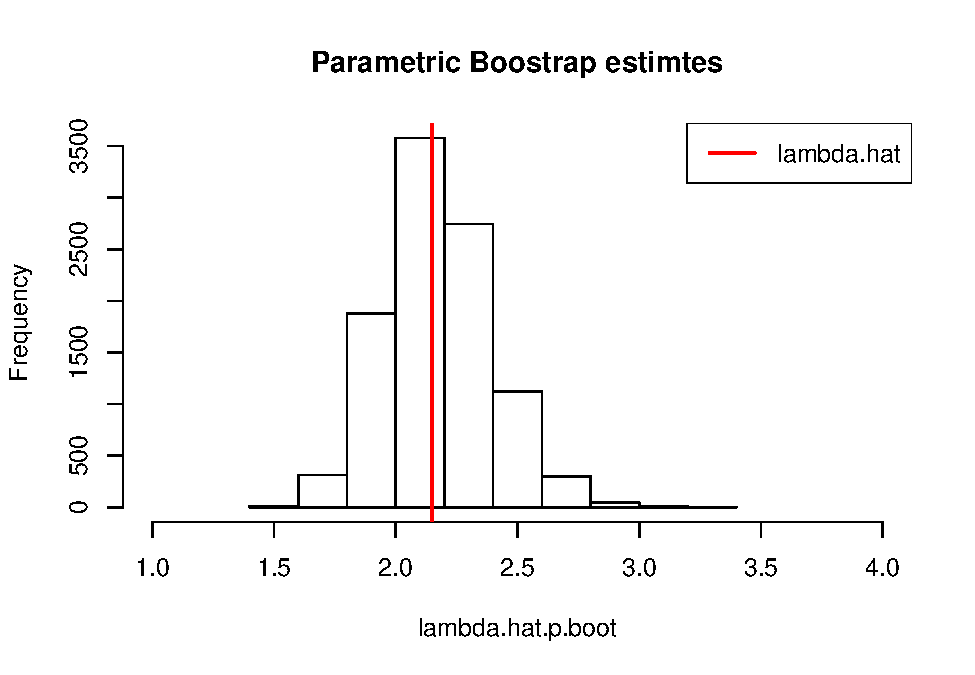
\includegraphics{Stats406Lab11_files/figure-latex/unnamed-chunk-5-1.pdf}

Bias is no cause for worry; variance is large at this sample size.

\subsection{Example 2: Non-parametric
bootstrap}\label{example-2-non-parametric-bootstrap}

We now perform the non-parametric version of bootsreap. No new data
points are simulated in this case.

\begin{Shaded}
\begin{Highlighting}[]
\NormalTok{lambda.hat.np.boot =}\StringTok{ }\KeywordTok{c}\NormalTok{() }
\NormalTok{for (i in }\DecValTok{1}\NormalTok{:B)\{}
    \NormalTok{sample.id =}\StringTok{ }\KeywordTok{sample}\NormalTok{(n,}\DataTypeTok{size=}\NormalTok{n, }\DataTypeTok{replace=}\OtherTok{TRUE}\NormalTok{)}
    \NormalTok{lambda.hat.np.boot[i] =}\StringTok{ }\NormalTok{n/}\KeywordTok{sum}\NormalTok{(x[sample.id]*y[sample.id])}
\NormalTok{\}}
\CommentTok{# bias}
\KeywordTok{mean}\NormalTok{(lambda.hat.np.boot)-lambda.hat}
\end{Highlighting}
\end{Shaded}

\begin{verbatim}
## [1] 0.01729434
\end{verbatim}

\begin{Shaded}
\begin{Highlighting}[]
\CommentTok{# variance}
\KeywordTok{var}\NormalTok{(lambda.hat.np.boot)}
\end{Highlighting}
\end{Shaded}

\begin{verbatim}
## [1] 0.04142713
\end{verbatim}

\begin{Shaded}
\begin{Highlighting}[]
\CommentTok{# MSE}
\KeywordTok{mean}\NormalTok{((lambda.hat.np.boot -}\StringTok{ }\NormalTok{lambda.hat)^}\DecValTok{2}\NormalTok{)}
\end{Highlighting}
\end{Shaded}

\begin{verbatim}
## [1] 0.04172209
\end{verbatim}

\begin{Shaded}
\begin{Highlighting}[]
\KeywordTok{hist}\NormalTok{(lambda.hat.np.boot, }\DataTypeTok{breaks =} \DecValTok{10}\NormalTok{, }\DataTypeTok{xlim =} \KeywordTok{c}\NormalTok{(}\DecValTok{1}\NormalTok{, }\DecValTok{4}\NormalTok{), }\DataTypeTok{main =} \StringTok{"Non-parametric Boostrap estimtes"}\NormalTok{)}
\KeywordTok{abline}\NormalTok{(}\DataTypeTok{v =} \NormalTok{lambda.hat, }\DataTypeTok{lwd =} \DecValTok{2}\NormalTok{, }\DataTypeTok{col =} \DecValTok{2}\NormalTok{)}
\KeywordTok{legend}\NormalTok{(}\StringTok{"topright"}\NormalTok{, }\DataTypeTok{legend =} \StringTok{"lambda.hat"}\NormalTok{, }\DataTypeTok{col =} \DecValTok{2}\NormalTok{, }\DataTypeTok{lwd =} \DecValTok{2}\NormalTok{, }\DataTypeTok{border =} \NormalTok{F)}
\end{Highlighting}
\end{Shaded}

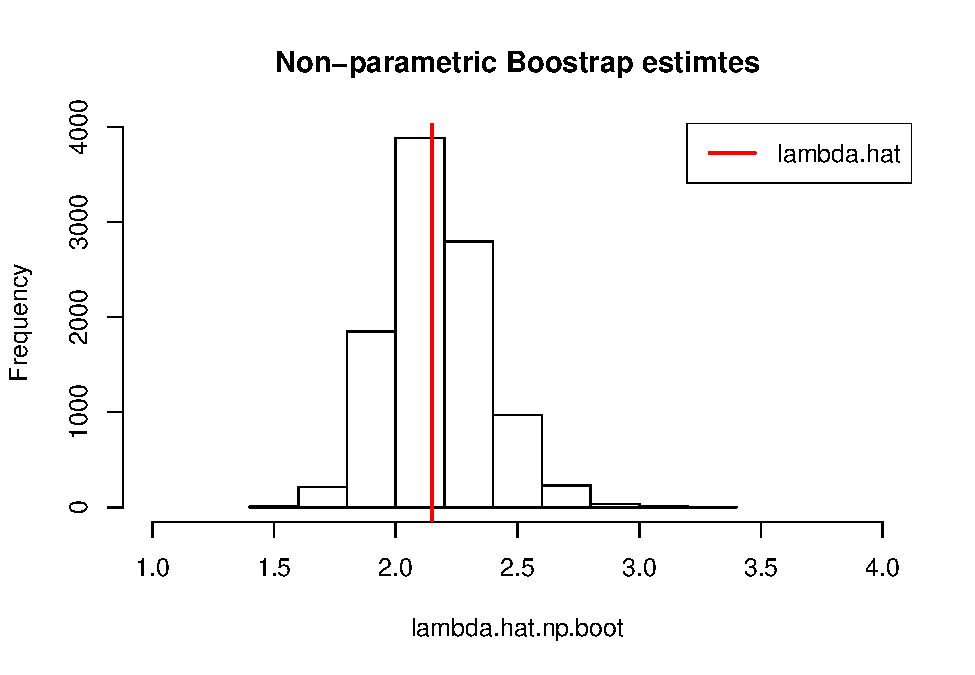
\includegraphics{Stats406Lab11_files/figure-latex/unnamed-chunk-6-1.pdf}

\subsection{Example 3 (optional): Treating design as
random}\label{example-3-optional-treating-design-as-random}

If we treat x input as realizations of random variable - i.e., random
design, we \emph{do} model x. To perform \emph{parametric} bootstrap of
\(\hat\lambda\) using \(y_i\) condition on \(x_i\), i = 1, \ldots{}, n,
we have to use nonparametric bootstrap to sample for \(x\)'s (there's no
way to perform parametric bootstrap to sample x since the distribution
of x is completely unspecified).

\begin{Shaded}
\begin{Highlighting}[]
\NormalTok{lambda.hat.p.np.boot =}\StringTok{ }\KeywordTok{c}\NormalTok{()}
\NormalTok{for (i in }\DecValTok{1}\NormalTok{:B)\{}
    \NormalTok{y.sample =}\StringTok{ }\KeywordTok{c}\NormalTok{()}
    \NormalTok{x.sample =}\StringTok{ }\KeywordTok{sample}\NormalTok{(x, }\DataTypeTok{size=}\NormalTok{n, }\DataTypeTok{replace=}\OtherTok{TRUE}\NormalTok{)}
    \NormalTok{y.sample =}\StringTok{ }\KeywordTok{sapply}\NormalTok{(lambda.hat*x.sample, }\DataTypeTok{FUN =} \NormalTok{function(x) }\KeywordTok{rexp}\NormalTok{(}\DecValTok{1}\NormalTok{,x))}
    \NormalTok{lambda.hat.p.np.boot[i] =}\StringTok{ }\NormalTok{n/}\KeywordTok{sum}\NormalTok{(x.sample*y.sample)}
\NormalTok{\}}
\CommentTok{# bias}
\KeywordTok{mean}\NormalTok{(lambda.hat.p.np.boot)-lambda.hat}
\end{Highlighting}
\end{Shaded}

\begin{verbatim}
## [1] 0.02234442
\end{verbatim}

\begin{Shaded}
\begin{Highlighting}[]
\CommentTok{# variance}
\KeywordTok{var}\NormalTok{(lambda.hat.p.np.boot)}
\end{Highlighting}
\end{Shaded}

\begin{verbatim}
## [1] 0.04773763
\end{verbatim}

\begin{Shaded}
\begin{Highlighting}[]
\CommentTok{# MSE}
\KeywordTok{mean}\NormalTok{((lambda.hat.p.np.boot -}\StringTok{ }\NormalTok{lambda.hat)^}\DecValTok{2}\NormalTok{)}
\end{Highlighting}
\end{Shaded}

\begin{verbatim}
## [1] 0.04823213
\end{verbatim}

\begin{Shaded}
\begin{Highlighting}[]
\KeywordTok{hist}\NormalTok{(lambda.hat.p.np.boot, }\DataTypeTok{breaks =} \DecValTok{10}\NormalTok{, }\DataTypeTok{xlim =} \KeywordTok{c}\NormalTok{(}\DecValTok{1}\NormalTok{, }\DecValTok{4}\NormalTok{), }\DataTypeTok{main =} \StringTok{"Boostrap estimtes under random design"}\NormalTok{)}
\KeywordTok{abline}\NormalTok{(}\DataTypeTok{v =} \NormalTok{lambda.hat, }\DataTypeTok{lwd =} \DecValTok{2}\NormalTok{, }\DataTypeTok{col =} \DecValTok{2}\NormalTok{)}
\KeywordTok{legend}\NormalTok{(}\StringTok{"topright"}\NormalTok{, }\DataTypeTok{legend =} \StringTok{"lambda.hat"}\NormalTok{, }\DataTypeTok{col =} \DecValTok{2}\NormalTok{, }\DataTypeTok{lwd =} \DecValTok{2}\NormalTok{, }\DataTypeTok{border =} \NormalTok{F)}
\end{Highlighting}
\end{Shaded}

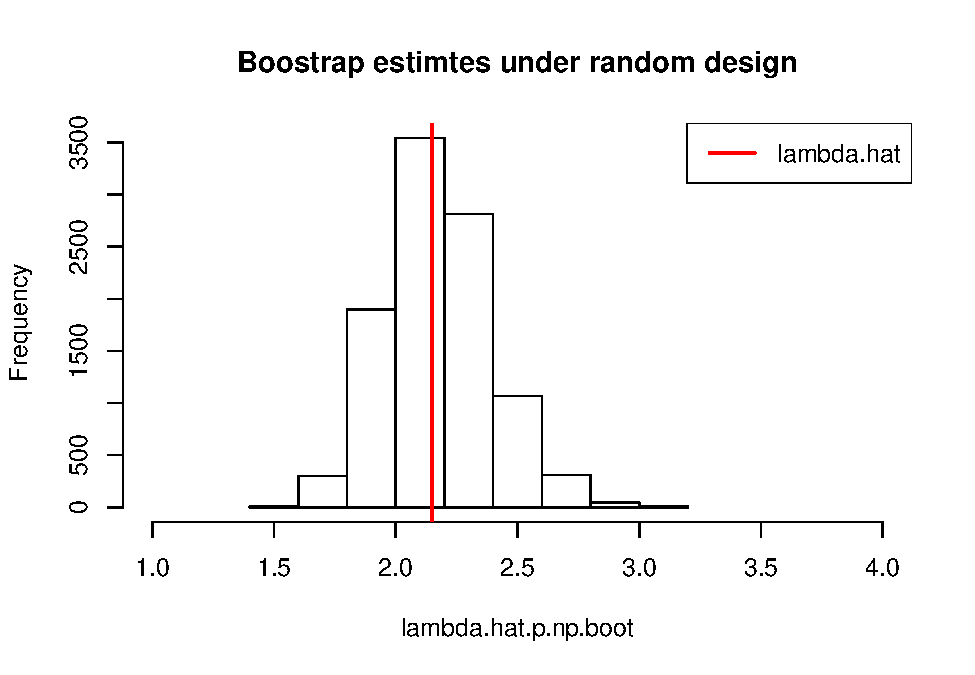
\includegraphics{Stats406Lab11_files/figure-latex/unnamed-chunk-7-1.pdf}

All three bootstrap estimates are pretty similar in this example.

\subsection{Extras}\label{extras}

When does bootstrap work? Bootstrap works in most applications and
perhaps all examples you will see in this course. The sufficient and
necesary condition for bootstrap consistency is that a central limit
property holds for \(\hat\theta\) (Mamman, 1992).

See more comprehensive treatment here
\url{http://www.unc.edu/~saraswat/teaching/econ870/fall11/JH_01.pdf}.


\end{document}
